\hoofdstuk{glossarium}


\begin{description}
\item[iOS]is a proprietary mobile operating system, developed by Apple Inc. It was originally released in 2007 for the iPhone and iPod Touch. iOS also became the main operating system of the iPad and Apple TV.

\cite{Sylvain2012}

\begin{centering}
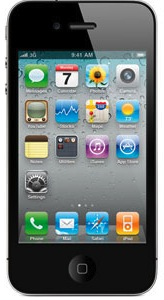
\includegraphics[scale=0.5]{images/iphone4.jpg}\\{4th generation Apple iPhone running iOS 4.3}\\
\end{centering}

\item[Android] is a open source mobile operating system, developed by the Open Handset Alliance, led by Google and other companies.\cite{Inc.2012}

\begin{centering}
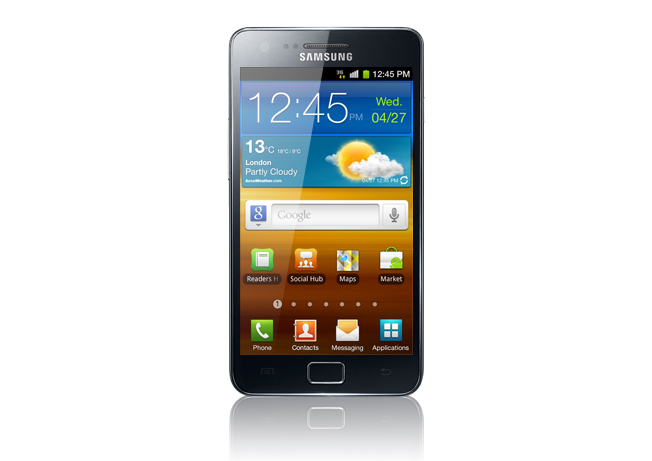
\includegraphics[scale=0.35]{images/android_sgs2.jpg}\\{Samsung Galaxy S2 running Android 2.3}\\
\end{centering}

% \subparagraaf{BlackBerry OS}
% BlackBerry OS is a proprietary mobile operating system, developed by RIM\emph{(Research In Motion)} for its line of BlackBerry mobile devices.

% \begin{centering}
% 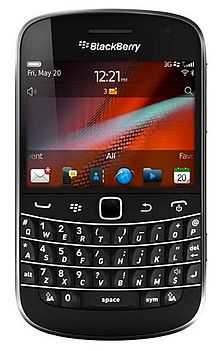
\includegraphics[scale=0.5]{images/Blackberrybold9900.jpg}\\{BlackBerry Bold 9900 running BlackBerry OS 7.1}\\
% \end{centering}


% \subparagraaf{Windows Phone 7}
% Windows Phone 7 is a mobile operating system developed by Microsoft as a succesor to its Windows Mobile platform.

% \begin{centering}
% 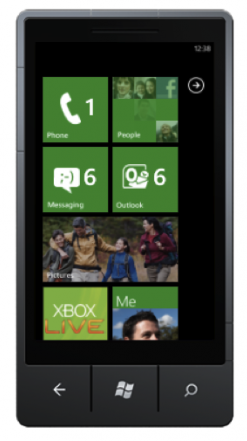
\includegraphics[scale=0.35]{images/WindowsPhone7.png}\\{Windows Phone 7}\\
% \end{centering}


% \subparagraaf{Other platforms}
% % Onder other valt Symbian. Symbian is een app platforms dus we nemen het mee:)
% \subparagraaf{Java ME}
% \subparagraaf{Symbian}

\item[i18n] is an a abbreviated numeronym of \emph{internationalization}, where 18 stands for the number of letters between the first i and last n in internationalization.
\end{description}